\subsubsection{Ažuriranje podataka klijenta od strane klijenta}

\begin{figure}[H]
\begin{center}
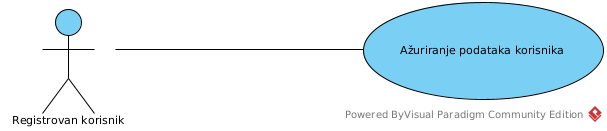
\includegraphics[width=\textwidth]{Pictures/uc_update_user_profile.png}
\end{center}
    \caption{Dijagram slučaja upotrebe ažuriranja podataka klijenta}
\label{fig:UCUpdateUserProfile}
\end{figure}

\begin{itemize}
    \item Kratak opis:
        \begin{itemize}
            \item Registrovani klijent ažurira svoje podatke putem aplikacije.
        \end{itemize}
    \item Učesnici:
        \begin{itemize}
            \item Registrovan klijent
        \end{itemize}
    \item Preduslovi:
        \begin{itemize}
            \item Sistem je u ispravnom stanju.
            \item Klijent mora biti registrovan i ulogovan na aplikaciju.
        \end{itemize}
    \item Postuslovi:
        \begin{itemize}
            \item Podaci su uspešno sačuvani u bazi podataka.
        \end{itemize}
    \item Osnovni tok:
        \begin{enumerate}
            \item Klijent bira opciju da ažurira svoje podatke.
            \item Sistem prikazuje formular za izmenu podataka.
            \item Klijent menja željene podatke. 
            \item Klijent bira opciju za čuvanje podataka.
            \item Sistem proverava da li su sva polja popunjena.
            \item Sistem čuva podatke i prikazuje poruku o uspešnosti.
        \end{enumerate}
    \item Alternativni tok:
        \begin{itemize}
            \item[5.a] Ukoliko sistem pronađe prazno polje, obeležava ga i obaveštava klijenta da sva polja moraju biti popunjena. Klijent popunjava polje. Proces se nastavlja u 4. koraku osnovnog toka.
        \end{itemize}
    \item Dodatne informacije:
        \begin{itemize}
            \item Podaci koji se mogu menjati su imejl adresa, lozinka i broj platne kartice.
        \end{itemize}
\end{itemize}

\begin{figure}[H]
\begin{center}
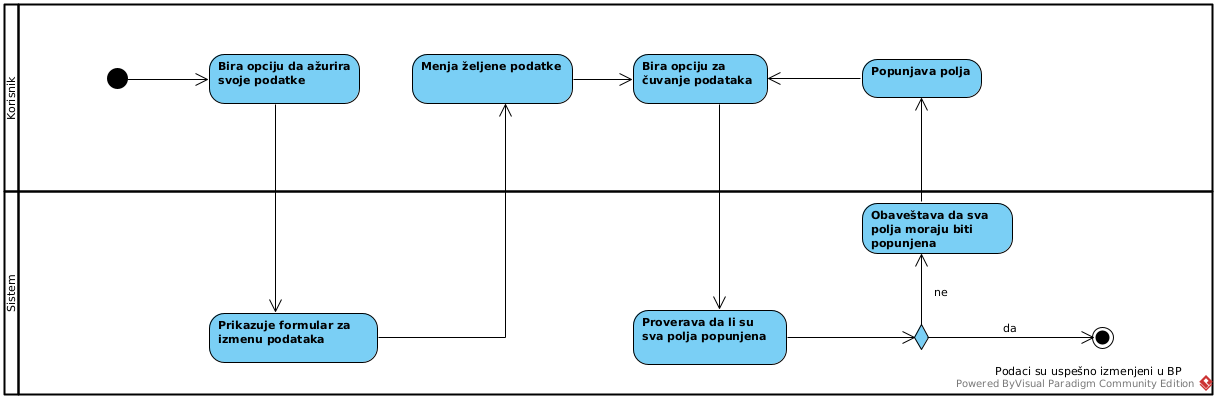
\includegraphics[width=\textwidth]{Pictures/activity_update_user_profile.png}
\end{center}
    \caption{Dijagram aktivnosti ažuriranja podataka klijenta}
\label{fig:ActivityUpdateUserProfile}
\end{figure}
